\documentclass[a4paper,12pt]{article}
\usepackage{polski}
\usepackage[polish]{babel}
\usepackage[utf8]{inputenc}
\usepackage{helvet}
\usepackage{graphicx}
\usepackage{color}
\usepackage{geometry}
\usepackage{epstopdf}
\usepackage{polski}
\usepackage{hyperref}
\usepackage{url}
\usepackage{indentfirst}
\newenvironment{bottompar}{\par\vspace*{\fill}}{\clearpage}
\geometry{hmargin={2cm, 2cm}, height=10.0in}
\usepackage[toc,page]{appendix}
\addto\captionspolish{%
  \renewcommand{\tablename}{Tabela}%
}

\begin{document}

% =====  STRONA TYTULOWA PRACY INŻYNIERSKIEJ ====
% ostatnia modyfikacja: 2011/03/09, K. Malarz

\thispagestyle{empty}

%% ------------------------ NAGLOWEK STRONY ---------------------------------

\includegraphics[height=37.5mm]{res/agh.eps}\\

\rule{30mm}{0pt}
{\large\textsf{Wydział Fizyki i Informatyki Stosowanej}}\\
\rule{\textwidth}{3pt}\\
\rule[2ex]
{\textwidth}{1pt}\\
\vspace{7ex}
\begin{center}
{\bf\LARGE\textsf{Praca inżynierska}}\\
\vspace{13ex}
% --------------------------- IMIE I NAZWISKO -------------------------------
{\bf\Large\textsf{Paweł Pęksa}}\\
\vspace{3ex}
{\sf \small kierunek studiów:} {\bf\small\textsf{informatyka stosowana}}\\
\vspace{15ex}
%% ------------------------ TYTUL PRACY --------------------------------------
{\bf\huge\textsf{Wykorzystanie algorytmów uczenia maszynowego w celu rozpoznawania nastroju muzyki}}\\
\vspace{14ex}
%% ------------------------ OPIEKUN PRACY ------------------------------------
{\sf \Large Opiekun:} {\bf\Large\textsf{dr hab. Marcin Wolter}}\\
\vspace{22ex}
\textsf{\bf\large\textsf{Kraków, styczeń 2016}}
\end{center}
%% =====  STRONA TYTUŁOWA PRACY INŻYNIERSKIEJ  ====

\newpage

%% =====  TYŁ STRONY TYTUŁOWEJ PRACY INŻYNIERSKIEJ  ====
{\sf Oświadczam, świadomy odpowiedzialności karnej za poświadczenie nieprawdy, że niniejszą pracę dyplomową wykonałem osobiście i samodzielnie i nie korzystałem ze źródeł innych niż wymienione w pracy.}

\vspace{14ex}

\begin{center}
\begin{tabular}{lr}
~~~~~~~~~~~~~~~~~~~~~~~~~~~~~~~~~~~~~~~~~~~~~~~~~~~~~~~~~~~~~~~~~ &
................................................................. \\
~ & {\sf (czytelny podpis)} \\
\end{tabular}
\end{center}

%% =====  TYL STRONY TYTULOWEJ PRACY INŻYNIERSKIEJ  ====

\newpage
\linespread{1.3}
\selectfont

\noindent


\vspace{85mm}
Merytoryczna ocena pracy przez opiekuna:
\begin{bottompar}
\begin{minipage}[t]{7cm}
\flushleft
Ocena: .........................

Data: ...........................
\end{minipage}
\hfill
\begin{minipage}[t]{7cm}
\flushright

Podpis: ........................
\end{minipage}
\end{bottompar}

\newpage



\vspace{85mm}
\noindent
Merytoryczna ocena pracy przez recenzenta:\\

\begin{bottompar}

\begin{minipage}[t]{7cm}
\flushleft
Ocena: .........................

Data: ...........................
\end{minipage}
\hfill
\begin{minipage}[t]{7cm}
\flushright

Podpis: ........................
\end{minipage}
\end{bottompar}

\newpage


%%%%%%%%%%%%%%%%%%%%%%%%%%%%%%%%%%%%%%%%%%%%%%%%%%%%%%%%%%%%%%%%%%%%%%%%%%%%%%%%%%%%%%%%%%%%%%%%%%%%%%%%%
%%%%%%%%%%%%%%%%%%%%%%%%%%%%%%%%%%%%%%%%%%%%%%%%%%%%%%%%%%%%%%%%%%%%%%%%%%%%%%%%%%%%%%%%%%%%%%%%%%%%%%%%%
%%%%%%%%%%%%%%%%%%%%%%%%%%%%%%%%%%%%%%%%%%%%%%%%%%%%%%%%%%%%%%%%%%%%%%%%%%%%%%%%%%%%%%%%%%%%%%%%%%%%%%%%%
%podziękowania

\begin{bottompar}

\begin{minipage}[t]{7cm}
\flushleft

\end{minipage}
\hfill
\begin{minipage}[t]{8cm}
\flushright
\noindent
\emph {Składam serdeczne podziękowania\\
Panu dr hab. Marcinowi Wolterowi\\
za udzieloną pomoc i poświęcony czas.}
\vspace{2cm}
\end{minipage}
\end{bottompar}

% spis tresci
\tableofcontents
\clearpage

\section{Wprowadzenie}
\subsection{Przedmiot pracy}
% music emotion recognition: sttate of the art review
Muzyka towarzyszyła człowiekowi od czasów prehistorycznych. Z~czasem stała się jedną z~form sztuki. Niewątpliwie, gdy słyszymy jakaś melodię, nie sprawia nam większego kłopotu, aby określić emocje z nią związane. Należy jednak mieć na uwadze źródło emocji. Rozróżnić możemy emocje wyrażane przez muzykę oraz przez nią indukowane. Tematem niniejszej pracy jest rozpoznawanie nastroju muzyki przy użyciu uczenia maszynowego. Przez określenie ,,nastrój muzyki'' mamy tutaj na myśli emocje, które ta muzyka reprezentuje. 
% W dalszej części pracy określenia "nastrój" odraz "emocje" będą używane naprzemiennie. 
Konkretnym narzędziem wybranym w celu klasyfikacji muzyki jest sztuczna sieć neuronowa. Idea klasyfikacji utworów muzycznych pod tym kątem jest względnie nowa, lecz można zauważyć wzrastające zainteresowanie tym tematem\cite{stateOfArt}. Do tej pory powstał szereg różnych prac podejmujących to zadanie\cite{musicANN1}\cite{musicANN2}\cite{musicANN3}. Niektóre korzystają nie tylko z samego sygnału audio, ale także np. z tekstu utworu\cite{musicLyrics}. W tej pracy jednak pod uwagę brany jest jedynie sygnał audio z~którego wyekstrahowano odpowiednie cechy, które mogłyby pozwolić sieci neuronowej rozpoznawać emocje reprezentowane przez dany utwór muzyczny. 
%Celem pracy jest stworzenie sztucznej sieci neuronowej, która będzie z powodzeniem potrafiła rozpoznawać nastrój %utworu bazując na wyekstrahowanych cecha utworu.

W kolejnych rozdziałach zostały opisane niezbędne podstawy teoretyczne, których przyswojenie pozwala zrozumieć w~jaki sposób postawione zadanie jest realizowane. W rozdziale \ref{rozdzial_sieci} znajduje się krótki opis sieci neuronowych, w rozdziale \ref{rozdzial_ekstrakcja} czytelnik dowie się o tym jakie konkretnie atrybuty muzyki były rozważane, natomiast w rozdziale \ref{rozdzial_modelEmocji} opisany jest sposób w~jaki matematyka pomaga nam w~opisaniu emocji. Opis stworzonego systemu można znaleźć w rozdziale \ref{rozdzial_system}. Wyniki oraz wnioski wynikające z podjętej próby podejścia do opisywanego zagadnienia zostały przedstawione w rozdziale kolejno \ref{rozdzial_wyniki} oraz \ref{rozdzial_wnioski}.
\subsection{Problematyka pracy}
Analiza muzyki pod kątem emocji jest zadaniem, które nie wiąże się tylko z przetwarzaniem sygnałów oraz uczeniem maszynowym, ale także z psychologią muzyki oraz jej teorią. Jest to bardzo wymagający problem, gdyż nastrój utworu muzycznego może być wysoce subiektywnym odczuciem. Wpływ na ocenę mogą mieć także wspomnienia danej osoby, nastrój w~danej chwili, indywidualne preferencje czy poziom wykształcenia muzycznego. Wszystkie wspomniane jednak kwestie nie są na tyle znaczące, aby podjęcie pracy nad tym tematem było niemożliwe czy całkowicie nieskuteczne. Oczywiście nie da stworzyć się systemu, który będzie działał niezawodnie, bo tak jak zostało to wspomniane, zbyt wiele indywidualnych czynników ma wpływ na percepcje człowieka. Dotychczasowe badania udowadniają, że jest możliwe sprostanie temu zadaniu w zadowalającym stopniu\cite{stateOfArt} i~taka próba zostaje podjęta w~niniejszej pracy.
% źródła: 
% Tadeusiewicz - Sieci Neuronowe
% http://www.cogsys.wiai.uni-bamberg.de/teaching/ws1112/km/practice/ANNs.pdf
% brief introduction to neural networks david kriesel
% http://neuralnetworksanddeeplearning.com

% default activate function: TanSig 
% default tarin function -> Gradient descent with momentum backpropagation and adaptive lr, hiperbolic tangent
\section{Sztuczne sieci neuronowe}\label{rozdzial_sieci}
Sztuczną siecią neuronową, dalej zwaną po prostu siecią neuronową, określamy model matematyczny służący jako system przetwarzania informacji. Źródłem inspiracji dla tegoż modelu była biologia, a~mianowicie sieci neuronowe istniejące w~ludzkim mózgu. Dużą zaletą sieci neuronowych jest fakt, iż nie działają jak tradycyjne algorytmy, lecz mają one zdolność do uczenia się. Jest to kolejna analogia związana z pracą ludzkiego mózgu, co powodowało wzrastające zainteresowanie tym tematem. Pomimo tego, że nie udało się z ich pomocą odtworzyć pracy tego niewątpliwie niesamowitego narządu, znajdują one zastosowanie w wielu dziedzinach nauki. Najbardziej podstawowym rodzajem sieci neuronowej jest sieć jednokierunkowa tj. czyli taka, w której nie występują sprzężenia zwrotne i~takie też sieci są wykorzystane w~tej pracy oraz opisane w~tym rozdziale.

%„Neuron McCullocha-Pittsa” autorstwa Wersję rastrową wykonał użytkownik polskiego projektu wikipedii: Andrut, Zwektoryzował: Krzysztof Zajączkowski - Wersja rastrowa: http://pl.wikipedia.org/wiki/Plik:Neuron_McCullocha-Pittsa.png. Licencja CC BY-SA 2.5 na podstawie Wikimedia Commons - https://commons.wikimedia.org/wiki/File:Neuron_McCullocha-Pittsa.svg#/media/File:Neuron_McCullocha-Pittsa.svg
%
\subsection{Budowa sieci neuronowej}
Szczegółowy opis zagadnień związanych z budową sieci neuronowej można znaleźć w pracy \cite{tadeusiewicz}.
\subsubsection{Budowa neuronu}
Sieć neuronowa zbudowana jest z~neuronów, które są odpowiednikami komórek nerwowych. Synapsy łączące poszczególne komórki modelowane są przez wagi liczbowe, których wielkości z kolei można interpretować jako wpływ jednej komórki na drugą. Matematyczny model neuronu użyty w sieciach neuronowych jest przedstawiony na rysunku \ref{neuron}. Składa się on z~$n+1$ wejść oraz jednego wyjścia. Dodatkowym wejściem neuronu jest tzw. bias, który przyjmuje stałą wartość, ale jest także modyfikowany w procesie uczenia (podobnie jak pozostałe wagi). Najczęściej przyjmuje się, że przed rozpoczęciem uczenia jego wartość równa jest $1$. Zależność pomiędzy sygnałami wejściowymi $x_i$, wagami $w_i$, a~tzw. sygnałem sumarycznego pobudzenia $\varphi$, w najprostszym przypadku może być określana przez wzór:
\begin{equation}
\varphi=w_0 + \sum_{i=1}^{n}w_i x_i.
\end{equation}
Sposób obliczenia sygnału wyjściowego neuronu określany jest przez funkcję aktywacji:
\begin{equation}
y=f(\varphi).
\end{equation}
Powszechnie używa się czterech funkcji aktywacji: funkcji liniowej, funkcji sigmoidalnej, funkcji tangens hiperboliczny oraz funkcji Gaussa\cite{leksykon}. Wzory poszczególnych funkcji znajdują się w~tabeli \ref{table:activation}, natomiast na rysunku \ref{funkcje} przedstawione zostały ich wykresy.

\begin{table}
\centering
\begin{tabular}{|c|c|}
\hline
funkcja & wzór \\
 \hline
liniowa  & $y=x$ \\  
 \hline
sigmoidalna  & $y=\frac{1}{1+e^{-x}}$ \\  
 \hline  
tangensoidalna  & $y = \frac{1-e^{-2x}}{1+e^{-2x}}$ \\  
\hline 
Gaussa & $e^{-x^2}$\\  
\hline 
 \end{tabular}
 \caption{Funkcje aktywacji wraz z ich wzorami} \label{table:activation}
\end{table}

\begin{figure}[ht!]
\centering
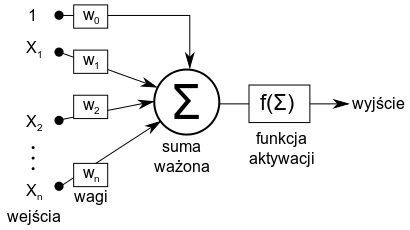
\includegraphics{res/neuron.png}
\caption[Caption for LOF]{Matematyczny model neuronu\label{neuron}\footnotemark}
% \caption{Matematyczny model neuronu\label{neuron} Źródło:\footnote{aa} } 
\end{figure} 


%obrazek z leksykonu
\begin{figure}[ht!]
\centering
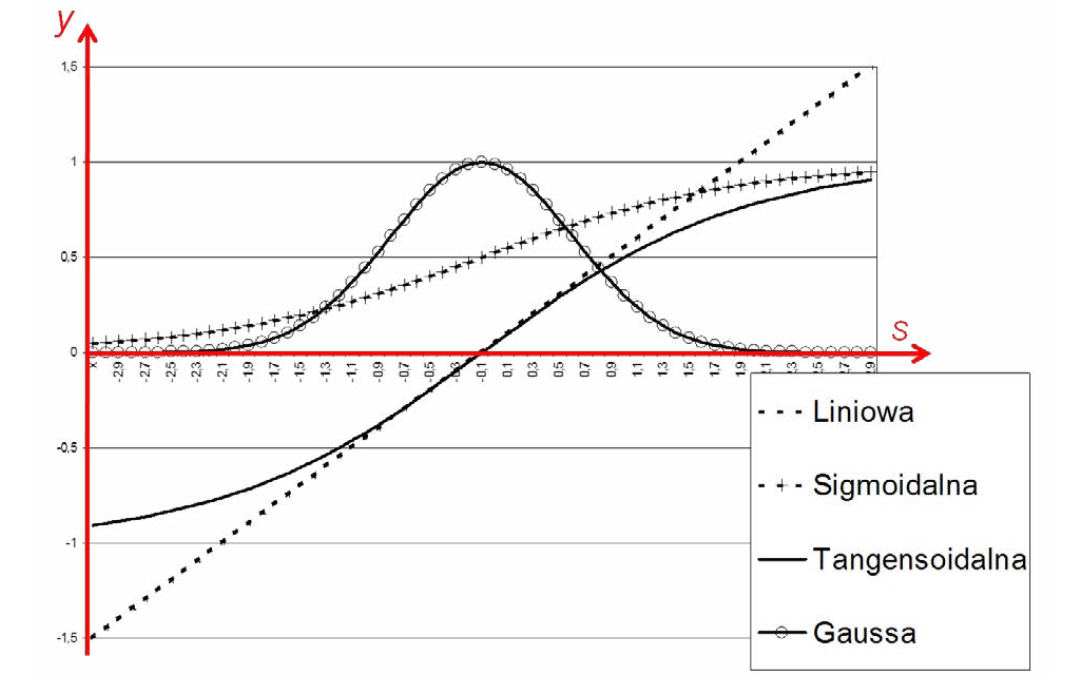
\includegraphics[scale=0.45]{res/funkcje.png}
\caption{Najczęściej używane funkcje aktywacji\cite{leksykon}\label{funkcje}}
\end{figure} 

\subsubsection{Topologia sieci}
\footnotetext{\url{http://pl.wikipedia.org/wiki/Plik:
Neuron_McCullocha-Pittsa.png}}
\begin{minipage}[adjusting]{\textwidth}
Wszystkie neurony zgrupowane są w warstwy z których możemy wyróżnić:
\begin{itemize}
\item warstwę wejściową
\item jedną lub więcej warstw ukrytych
\item warstwę wyjściową
\end{itemize}
\end{minipage}\vspace{1cm}
W~każdej z~warstw znajduje się dowolna liczba neuronów, który posiada połączenie do wszystkich neuronów znajdujących się w~warstwie kolejnej. Przykład sieci neuronowej składającej się z~dokładnie trzech warstw zawierającej różną ilość neuronów w każdej z~nich został przedstawiony na rysunku \ref{net}.

\begin{figure}[ht!]
\centering
% obrazek pobrany z 
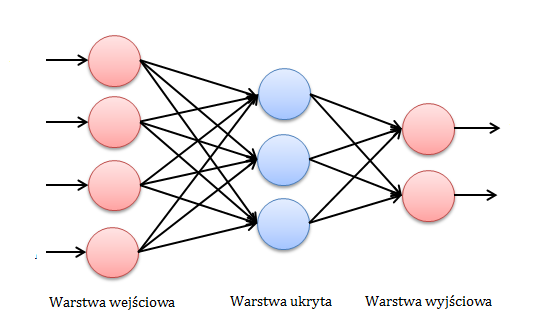
\includegraphics{res/exampleNet.png}
\caption[Caption for LOF]{Przykładowa jednokierunkowa sieć neuronowa\label{net}\footnotemark} 
\end{figure}
\footnotetext{\url{https://2ml4pa.bn1303.livefilestore.com/y2p6no6Dn0weHW3FG9tceTUS9lohx5ldcxvFZRhKdbeFQi2kntad_77gKeKIC-INcsFRCvGI-_DY9lMdZzaX8jkSHDvqlcT3qRnftpAt7esi4s/1.PNG?psid=1}}
%Źródło:\url{https://2ml4pa.bn1303.livefilestore.com/y2p6no6Dn0weHW3FG9tceTUS9lohx5ldcxvFZRhKdbeFQi2kntad_77gKeKIC-INcsFRCvGI-_DY9lMdZzaX8jkSHDvqlcT3qRnftpAt7esi4s/1.PNG?psid=1}}

\subsection{Uczenie sieci neuronowej} 
Wyróżniamy dwa podstawowe sposoby uczenia sieci:
\begin{itemize}
\item uczenie z nauczycielem (uczenie nadzorowane) - gdy dysponujemy danym treningowymi
\item uczenie bez nauczyciela (uczenie nienadzorowane) - gdy nie dysponujemy danymi treningowymi, a~sieć neuronowa klasyfikuje dane znajdując podobieństwa pomiędzy przypadkami 
\end{itemize}
W~niniejszej pracy zastosowane zostało uczenie sieci z~nauczycielem. Dzięki możliwości uczenia sieci neuronowej nie jest konieczne projektowanie algorytmu, który przetwarza dla nas informacje w oczekiwany sposób. Sieć neuronowa korzystając z~odpowiedniego algorytmu uczenia sama modeluje ten algorytm poprzez modyfikację wag. Należy też wspomnieć, że początkowe wagi sieci neuronowej zwykle inicjalizowane są wartościami losowymi.   

\subsubsection{Reguła delta}
Proces uczenia polega na modyfikowaniu współczynników wagowych sieci neuronowej. Opisane w tym podrozdziale zostanie uczenie z~nauczycielem, ponieważ takie właśnie zostało wykorzystane w~tej pracy. W~przypadku uczenia z~nauczycielem potrzebujmy zbioru uczącego składającego się z~wektora danych, które podajemy na wejście sieci i~oczekiwanego rezultatu dla tego przypadku, co możemy oznaczyć jako pary $(y_i,z_i)$, gdzie $z_i$ jest oczekiwaną odpowiedzią dla sygnału wejściowego $x_i$. Zadaniem sieci jest modelowanie funkcji:
\begin{equation}
h(x)=z.
\end{equation}
Uczenie jest procesem iteracyjnym, gdzie w~każdej iteracji modyfikujemy wagi sieci. Liczba iteracji $N$ równa jest liczbie par $(x_i,z_i)$. W~każdym kroku $j$ procesu uczenia możemy zdefiniować wielkość błędu neuronu wyjściowego jako:
\begin{equation}
\delta_i^j = |z_i^j - y_i^j|,
\end{equation}
gdzie $y_i$ jest odpowiedzią sieci neuronowej dla sygnału $x_i$.
Proces uczenia jest realizowany poprzez minimalizację funkcji:
\begin{equation}\label{minFunc}
Q=\frac{1}{2}\sum_{j=1}^{N}(\delta_i)^2
\end{equation}
będącej miarą dopasowania funkcji metodą najmniejszych kwadratów. Korzystając z metody gradientowej możemy zdefiniować poprawkę $\Delta w$ dla wagi $w$ neuronu $i$ jako:
\begin{equation}\label{deltaRule}
\Delta w_i = - \eta \frac{\partial Q}{\partial w_i},
\end{equation}
oraz, idąc dalej, zdefiniować wzór korygujący wagi $w$ w kolejnych krokach:
\begin{equation}
w^{j+1}_i = w^j_i + \Delta w_i
\end{equation}
przy czym $\eta$ jest dodatkowym współczynnikiem liczbowym, który decyduje o szybkości uczenia. W ten sposób poprawiamy wagi sieci $j$ razy. Problemem z~którym borykano się do połowy lat 80-tych jest fakt, iż tym sposobem niemożliwe jest uczenie sieci, która składa się z~więcej niż jednej warstwy, ponieważ nieznana jest oczekiwana odpowiedź neuronów warstwy innej niż wyjściowej. Wzór \ref{deltaRule} jest jednak podstawą większości algorytmów automatycznego uczenia\cite{tadeusiewicz} i~jest on określany w literaturze regułą delta\cite{briefIntroduction}.

\subsubsection{Algorytm wstecznej propagacji błędów}
W~celu przeprowadzenia uczenia dla sieci wielowarstwowej spotykamy się z~potrzebą określenia błędu $\delta$ dla neuronów, które należą do warstw ukrytych sieci neuronowej. Umożliwia nam to algorytm wstecznej propagacji błędów. Błąd dla takiego neuronu obliczamy korzystając ze wszystkich błędów neuronów do których wysłał on swój sygnał. Uwzględniane są także wagi połączeń. Mowa jest o wstecznej propagacji, ponieważ odbywa się ona przeciwnie do przepływów sygnałów w~sieci. Błąd dla neuronów znajdujących się w~warstwie innej niż wejściowa możemy określić jako:
\begin{equation}
\delta_i = f'(\varphi) \sum_{i}^{N}w_k \delta _k,
\end{equation}
przy czym $w_k$ oraz $\delta _k$ są kolejno wagami oraz błędami neuronów do których analizowany neuron wysyłał swój sygnał.
%Korzystając z definicji pochodnej złożonej - biorąc pod uwagę, że $Q$ zależy od $y$, a $y$ od $w$ - możemy %zapisać wzór \ref{deltaRule} jako:
%\begin{equation}
%\Delta w = - \eta \frac{\partial Q}{\partial y} \frac{\partial y}{\partial w}
%\end{equation}
%biorąc pod uwagę:
%\begin{equation}
%frac{\partial Q}{\partial y} = - \delta
%end{equation}
\section{Ekstrakcja cech dźwiękowych}\label{rozdzial_ekstrakcja}
Cechami dźwiękowymi nazywamy zmienne wyekstrahowane z~sygnału audio, które opisują ten sygnał i~pozwalają uzyskać dodatkowe informacje na jego temat\cite{phdWork}. Opisane w~tym rozdziale zostały cechy sygnału audio, które są wejściami dla użytego klasyfikatora tj. sieci neuronowej. Poszczególne cechy bazowały zarówno na czasowej jak i~spektralnej reprezentacji sygnału.

\subsection{Cyfrowa reprezentacja sygnału audio}
Dźwięk jest sygnałem analogowym. W~celu przechowywania go na cyfrowych nośnikach spotkano się z~potrzebą jego digitalizacji tj. reprezentacji w~postaci cyfrowej. Najczęściej stosowaną w~tym celu jest metoda PCM\footnote{PCM - Pulse Code Modulation}
w~której to sygnał analogowy jest próbkowany w równych odstępach czasu i~zapisywany cyfrowo. Powszechnie stosowana częstotliwość próbkowania wynosi 44 100~Hz ze względu na zakres częstotliwości słyszanych przez człowieka, który wynosi około 20 000~Hz, a~zgodnie z~prawem Nyquista sygnał powinien być próbkowany z~dwa razy wyższą częstotliwością niż maksymalna częstotliwość sygnału w celu uzyskania dokładnej reprezentacji bez zniekształceń\cite{signalProcessing}. Przykładowy, reprezentowany cyfrowo, sygnał audio przedstawia rysunek \ref{audioExample1} oraz \ref{audioExample2}. Na rysunku \ref{audioExample2} przedstawiony został ten sam sygnał, który widzimy na rysunku \ref{audioExample1}, lecz w bardzo dużym przybliżeniu. Oba rysunki zostały wygenerowane za pomocą programu Audacity\cite{audacity} z~pliku audio w~formacie mp3\footnote{Format cyfrowego zapisu i~kompresji plików dźwiękowych}.

\begin{figure}[ht!]
\centering
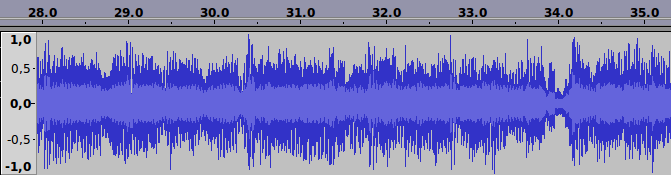
\includegraphics[scale=0.5]{res/exampleAudio1.png}
\caption{Przykładowy sygnał audio\label{audioExample1}}
\end{figure}

\begin{figure}[ht!]
\centering
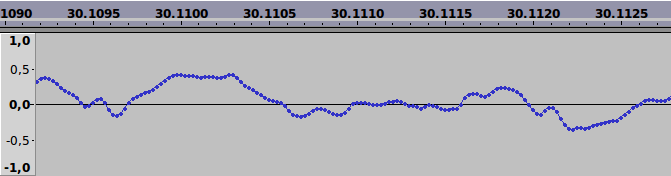
\includegraphics[scale=0.5]{res/exampleAudio2.png}
\caption{Przykładowy sygnał audio - przybliżenie\label{audioExample2}}
\end{figure}

\subsection{Spektralna reprezentacja sygnału audio}
\subsubsection{Transformacja Fouriera}
Każdy sygnał, który jest reprezentowany jako zmieniająca się w~czasie amplituda posiada też odpowiadające spektrum częstotliwościowe tzw. widmo. Dotyczy to także sygnału audio. Dzięki przedstawieniu sygnału dźwiękowego w~ten sposób możliwe jest uzyskanie dodatkowych informacji na jego temat\cite{windowingNI}. Spektrum przedstawia skład częstotliwościowy dźwięku. Przy obliczaniu spektrum z~pomocą przychodzi transformacja Fouriera. Oznaczając $x(t)$ jako sygnał, a~$X(f)$ jako wynik transformacji, możemy zapisać:
\begin{equation}
X(f)=\int\limits_{-\infty}^{\infty} x(t)e^{-j2\pi ft} dt ,
\end{equation}
przy czym $f$ to częstotliwość, natomiast $t$ oznacza czas. W~celu otrzymania spektrum amplitudowego, z~którego szeroko korzystano w~niniejszej pracy, należy z~otrzymanego wyniku obliczyć wartość bezwzględną:
\begin{equation}
|X(f)|.
\end{equation}
Trzeba jednak pamiętać, że w~przypadku sygnału audio zapisanego w~pamięci komputera mamy do czynienia z~sygnałem dyskretnym, więc należy użyć DFT\footnote{Discrete Fourier Transform} - transformaty Fouriera dla sygnałów dyskretnych wyrażającej się wzorem:
\begin{equation}
X_k = \sum_{n=0}^{N-1}x_n e^{-i2\pi\frac{k}{N}n} ,
\end{equation}
przy czym $x_n$ to kolejne wartości próbkowanego sygnału, $X_k$ to wartości transformaty. Na rysunku \ref{spectrumExample} przedstawiony jest przykładowy sygnał wraz z~odpowiadającym mu spektrum amplitudowym.

%https://en.wikipedia.org/wiki/Spectral_density#/media/File:Voice_waveform_and_spectrum.png
\begin{figure}[ht!]
\centering
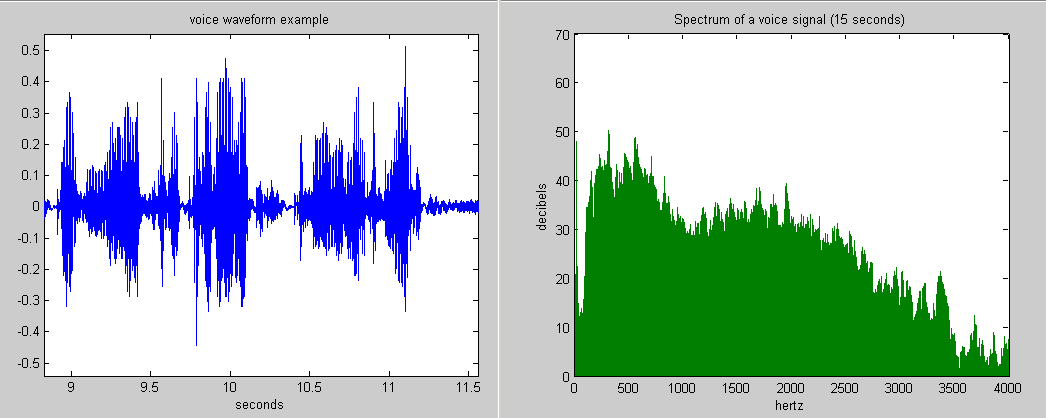
\includegraphics[scale=0.5]{res/spectrumExample.png}
\caption[Caption for LOF]{Sygnał audio wraz z odpowiadającym mu spektrum amplitudowym\label{spectrumExample} \footnotemark}
\end{figure}

\footnotetext{\url{https://commons.wikimedia.org/wiki/File:Voice_waveform_and_spectrum.png}}



\subsection{Wstępna obróbka sygnału}
Przed analizą sygnału dźwiękowego, jakim są utwory muzyczne, w~celu poprawy jakości danych przeprowadza się obróbkę wstępną, co pozwala na bardziej efektywną jego analizę. Przed ekstrakcją cech dźwiękowych wykorzystana została funkcja okna czasowego oraz algorytm wyrównywania poziomu głośności dźwięku opisane w~kolejnych dwóch podrozdziałach.

\subsubsection{Okno czasowe}
Ważną rolę przy korzystaniu z~transformaty Fouriera odgrywa okresowość. W~przypadku, gdy mamy do czynienia z~danymi, które występują niecałkowitą ilość razy, na końcach analizowanych danych występują nieciągłości, które powodują, że otrzymane spektrum jest zniekształcone. Rozwiązaniem tego problemu jest okno czasowe. Jest to funkcja, którą mnożymy przy sygnał w celu zmniejszenia zniekształceń\cite{windowingNI}. 

\subsubsection{Algorytm wyrównywania poziomu głośności dźwięku}
Ludzkie ucho nie słyszy dźwięków o~wszystkich częstotliwościach jako dźwięków o~tym samym poziomie głośności. Problem ten można rozwiązać częściowo przy użyciu algorytmu wyrównywania poziomu głośności, który filtruje dźwięk korzystając z~krzywych izofonicznych. Pojecie izofony lub też krzywej izofonicznej określa w fonach\footnote{Fon - jednostka poziomu głośności} słyszalne natężenie dźwięku w~zależności od częstotliwości\cite{izofona}. Ze względu na subiektywność postrzegania głośności nie istnieją ściśle określone krzywe izofoniczne. Istnieje jednak model zaproponowany przez Fletchera oraz Munsona\cite{izofonyModel}, który jest przedstawiony na rysunku \ref{izofony}.

%obrazek
% autor „FletcherMunson ELC” autorstwa Oarih - Created by Oarih using Inkscape. Licencja CC BY-SA 3.0 na podstawie Wikimedia Commons - https://commons.wikimedia.org/wiki/File:FletcherMunson_ELC.svg#/media/File:FletcherMunson_ELC.svg
\begin{figure}[ht!]
\centering
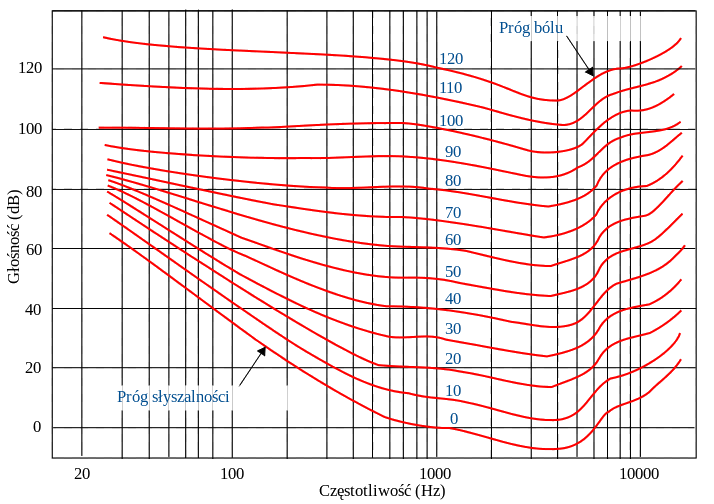
\includegraphics[scale=0.5]{res/equalLoudness.png}
\caption[Caption for LOF]{Izofony „normalnego” ucha według Fletchera i Munsona\footnotemark, wartości fonów dla poszczególnych krzywych określone są liczbami w kolorze niebieskim\label{izofony}
}
\end{figure}
\footnotetext{\url{https://commons.wikimedia.org/wiki/File:FletcherMunson_ELC.svg}}


\subsection{Cechy dźwięku bazujące na czasowej reprezentacji dźwięku}
W~niniejszym rozdziale zostały krótko opisane cechy dźwięku, które zostały rozważone w~pracy. W~kolejnych podrozdziałach oznaczono $f_i$ jako kolejne częstotliwości widma oraz $a_i$ jako odpowiadające im amplitudy.
\subsubsection{Wskaźnik zmiany znaku (\emph{Zero Crossing Rate})}
Wskaźnik zmiany znaku (\emph{Zero Crossing Rate}) jest jedną z~najprostszych cech dźwiękowych obliczanych z~wykorzystaniem reprezentacji dźwięku jako zmiana amplitudy w czasie. Wyraża on liczbę zmiany znaków w fali dźwiękowej w~jednostce czasu. Możemy określić go wzorem:
\begin{equation}
ZCR = \frac{1}{2} \sum^{N}_{n=1} |sgn(x[n]) - sgn(x[n-1])|.
\end{equation}
Jest to deskryptor często stosowany w~pozyskiwaniu informacji z~muzyki, ale także stosowany w~rozpoznawaniu mowy. Zawdzięcza to łatwości jego obliczania, a~także faktowi, że przechowuje informację o~szumach występujących w~dźwięku\cite{phdWork}.

\subsubsection{Wskaźnik zmian (\emph{Onset rate})}
Wskaźnik zmian (\emph{Onset rate}) jest podstawowym wskaźnikiem rytmu utworu muzycznego mającym duży wpływ na postrzeganie emocji reprezentowanych przez muzykę, ponieważ mówi o~zmienności dźwięku. Jest on określany jako liczba ekstremów obwiedni dźwięku\footnote{Krzywa opisująca zmianę amplitudy
sygnału\cite{obwiednia}}. Zakłada się, że różnica czasowa pomiędzy dwoma zmianami branym pod uwagę w~zliczaniu musi wynosić przynajmniej 60 ms\cite{phdWork}. 
 
\subsection{Cechy dźwięku bazujące na spektralnej reprezentacji dźwięku}
\subsubsection{Złożoność spektralna (\emph{Spectral complexity})}
Złożoność spektralna (\emph{spectral complexity}) jest liczbą ekstremów w~widmie amplitudowym sygnału dźwiękowego. Opisuje ona złożoność tego widma. Utwory z~większą średnią złożonością spektralną charakteryzują się większą energicznością\cite{phdWork}.

\subsubsection{Kształt spektralny (\emph{Spectral shape})}
Kształt spektralny jest kształtem widma amplitudowego danego sygnału dźwiękowego. W~jego skład wchodzą m.in. środek masy widma sygnału (\emph{spectral centroid}), współczynnik skośności widma sygnału (\emph{spectral skewness}), kurtoza widma sygnału (\emph{spectral kurtosis}), tzw. \emph{spectral roll-off} oraz rozrzut spektralny (\emph{spectral spread}). Wszystkie te cechy mają wpływ na odbiór utworu muzycznego przez słuchacza pod kątem reprezentowanych przez utwór emocji\cite{phdWork}.

\paragraph{Moment centralny}\mbox{}\\
W~celu określenia kolejnych wzorów mówiących o kształcie spektralnym użyteczne jest zdefiniowanie momentu centralnego. Dla zmiennej dyskretnej moment centralny jest przedstawia się wzorem:
\begin{equation}\label{momentCentralny}
\mu = \sum^{N}_{i=1} \frac{(f_i - \overline{f})^r}{N},
\end{equation}
gdzie $f_i$ są kolejnymi częstotliwościami występującymi w~widmie, $\overline{f}$ średnią częstotliwością, natomiast $N$ to liczba wszystkich częstotliwości. Moment centralny rzędu drugiego obliczamy korzystając ze wzoru \ref{momentCentralny}:
\begin{equation}
\sigma ^ 2 = \sum^{N}_{i=1} \frac{(f_i - \overline{f})^2}{N}
\end{equation}
i~nazywany wariancją. Pierwiastek kwadratowy z~wariancji $\sigma$ określany jest mianem odchylenia standardowego.

\paragraph{Środek masy widma}\mbox{}\\
Środek masy widma wyrażamy wzorem:
\begin{equation}
SC = \frac{\sum f_i a_i}{a_i},
\end{equation}
gdzie $f_i$ jest częstotliwością, natomiast $a_i$ amplitudą dla poszczególnych częstotliwości\cite{phdWork}.

\paragraph{Współczynnik skośności widma}\mbox{}\\
Współczynnik skośności mówi o~asymetryczności widma. W przypadku, gdy jest on mniejszy od zera, więcej danych znajduje się po lewej stronie widma, w przypadku, gdy jest on większy od zera, więcej danych znajduje się po prawej stronie widma. Określa się go wzorem:
\begin{equation}
\gamma = \frac{\mu _3 }{\sigma ^3}
\end{equation}

\paragraph{Kurtoza widma}\mbox{}\\
Kurtoza widma jest miarą jego spłaszczenia, wyraża się wzorem:
\begin{equation}
K = \frac{\mu _4 }{\sigma ^4}
\end{equation}

\paragraph{\emph{Roll-off} widma}\mbox{}\\
Cechą dźwięku określana mianem \emph{Roll-off}'u widma jest częstotliwość, która dzieli widmo sygnału na dwie części według ustalonego progu $T$, który zazwyczaj wynosi 0.95\cite{phdWork}. Omawiana cecha jest zdefiniowana wzorem\cite{rollOff}:
\begin{equation}
\sum_{i=1}^{R_t}f_i = T \sum_{i=1}^{N}f_i.
\end{equation}

\paragraph{Rozrzut spektralny}\mbox{}\\
Rozrzut spektralny jest miarą mówiącą o~szerokości widma sygnału, który wyraża się wzorem:
\begin{equation}
spectralSpread = \frac{\sum_{i}^{}(f_i - SC)^2 a_i}{\sum_{i}a_i} 
\end{equation}
Utwory muzyczne o większym rozrzucie spektralnym charakteryzują się większą energicznością. % cite?

\subsubsection{Płaskość spektralna \emph{(Spectral flatness)}}
Płaskość spektralna jest stosunkiem średniej arytmetycznej do średniej geometrycznej widma amplitudowego wyrażonym w decybelach:
\begin{equation}
spectralFlatness=10 log_{10} \frac{G}{A}
\end{equation}
przy czym $G$ jest średnią geometryczną:
\begin{equation}
G=\sqrt[n]{\prod_{i=1}^{N} a_i}
\end{equation}
oraz $A$ jest średnią arytmetyczną:
\begin{equation}
A=\frac{\sum_{i=1}^{N}a_i}{N}.
\end{equation}
Cecha ta określa jak bardzo spłaszczony jest wykres widma amplitudowego. Wraz ze wzrostem tego wskaźnika dźwięk bardziej przypomina szum. Wartość bliska 1 świadczy o występowaniu białego szumu\footnote{Szum akustyczny o prawie płaskim widmie}\cite{phdWork}.


\subsubsection{Dysonans (\emph{Dissonance})}
Dysonans jest deskryptorem dźwięku obliczanym na podstawie odstępów pomiędzy ekstremami widma amplitudowego. W~przypadku utworów muzycznych cechujących się mniejszym rozdźwiękiem obserwuje się większą równomierność tychże odstępów. Matematycznie dysonans można określić wzorem:
\begin{equation}
dissonance = \frac{1}{H}\sum_{h=1}^{H} a(h) - SE(h),
\end{equation}
gdzie $H$ jest liczbą ekstremów, $a(h)$ amplitudą dla danego ekstremum oraz $SE(h)$ amplitudą obwiedni spektrum dla częstotliwości $f(h)$\cite{phdWork}.

\subsubsection{Skala}
Skala muzyczna składa się z~dźwięków o~różnych częstotliwościach ułożonych według ustalonego schematu. Możemy wyróżnić dwie podstawowe skale: molową oraz durową. Powszechnie uznaje się, że utwory muzyczne bazujące na skali durowej mają radosne brzmienie, natomiast na skali molowej smutne brzmienie\cite{skala}. W~celu wyekstrahowania skali muzycznej utworu należy najpierw obliczyć jego HPCP\footnote{Harmonic Pitch Class Profile}, który obliczany jest na podstawie ekstremów widma amplitudowego według wzoru:
\begin{equation}
HPCP(n) = \sum^{N}_{i=1} w(n,f_i)a_i ^2,
\end{equation}
gdzie $a_i$ oraz $f_i$ są kolejno amplitudą oraz częstotliwością ekstremum, $N$ jest liczbą wszystkich ekstremów, $n$ kolejną wartością wektora HPCP, natomiast $w$ funkcją wagową określającą w jaki sposób poszczególne ekstremum wpływa na wartość $n$ wartości wektora HPCP. W celu określenia skali muzycznej obliczana jest korelacja pomiędzy wektorem HPCP, a odpowiednimi profilami dla obu skali\cite{hpcp}.










    

\section{Matematyczny model emocji}\label{rozdzial_modelEmocji}
W~celu realizacji postawionego zadania należy zdefiniować emocje matematycznie. Jednym z~podejść stosowanych w~pracach o~podobnej tematyce jest wykorzystanie etykiet mówiących o emocjach. Każdy z~utworów etykietowano z~wykorzystaniem przymiotników takich jak np. ,,smutny'', ,,wesoły'', ,,relaksujący''.  Innym rozwiązaniem jest określanie emocji z~wykorzystaniem dwuwymiarowej przestrzeni opracowanej przez Russell'a\cite{emotion} i~podobnie postąpiono w~niniejszej pracy. W~tym przypadku, emocje określona są przy pomocy dwóch parametrów: pobudzenia(ang. \emph{arousal}) oraz zadowolenia(ang. \emph{valence}), co przedstawia rysunek \ref{russelModel}. Model ten zakłada, że wszystkie emocje wynikają z~dwóch niezależnych systemów neurofizjologicznych\footnote{system neurofizjologiczny - system układu nerwowego} w~kontekście do poprzednich teorii zakładających istnienie niezależnych systemów dla każdej podstawowej emocji. Wyniki najnowszych badań są jednak bardziej konsystentne z~nowszym podejściem\cite{emotion}.

% https://www.researchgate.net/publication/258273035_The_physiological_Measurements_as_a_Critical_Indicator_in_Users'_Experience_Evaluation

\begin{figure}[ht!]
\centering
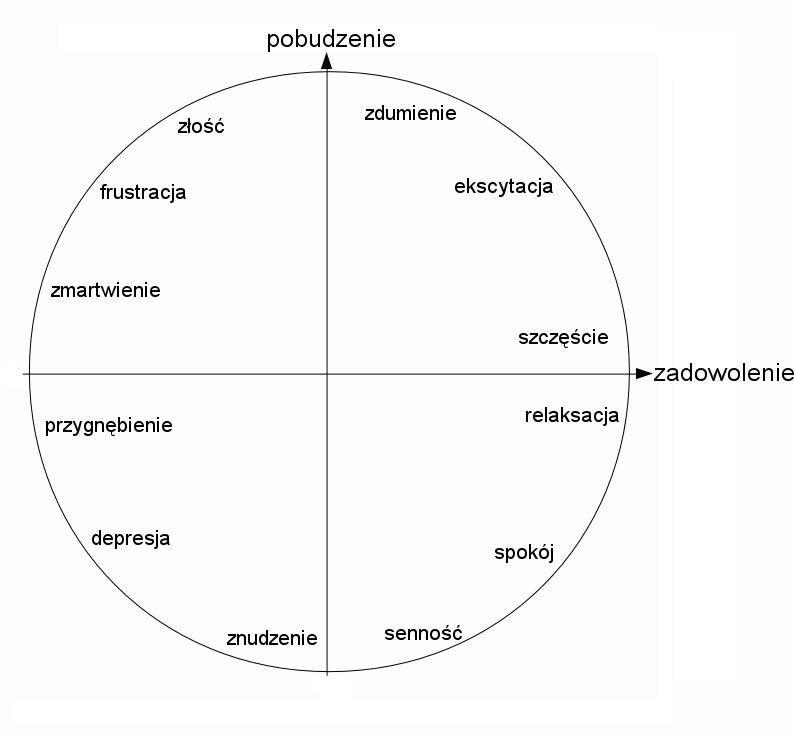
\includegraphics[scale=0.5]{res/emotionModel.png}
\caption{Model emocji według Russela}\label{russelModel}
\end{figure}
\section{Opis stworzonego systemu}\label{rozdzial_system}
W~niniejszym rozdziale opisana jest realizacja systemu stworzonego przez autora pracy. W kolejnych podrozdziałach znajdują się opisy poszczególnych jego elementów oraz użytych narzędzi.

\subsection{Schemat systemu}
Na rysunku \ref{systemSchemeImage} przedstawiony został schemat stworzonego systemu, który posłużył do realizacji klasyfikacji utworów muzycznych. Pokazuje on ogólny zamysł zaproponowany przez autora w~celu rozwiązania problemu rozpoznawania nastroju muzyki. Pierwszym krokiem, który należy podjąć jest wstępna obróbka utworów muzycznych, a~następnie wyekstrahowanie ich cech dźwięków. Na podstawie takie bazy danych należy podzielić dane na zbiór uczący oraz testowy, które będą służyć kolejno do uczenia sieci neuronowej, a~następnie do jej oceny przez klasyfikator, którym jest sieć neuronowa.

\begin{figure}[ht!]
\centering
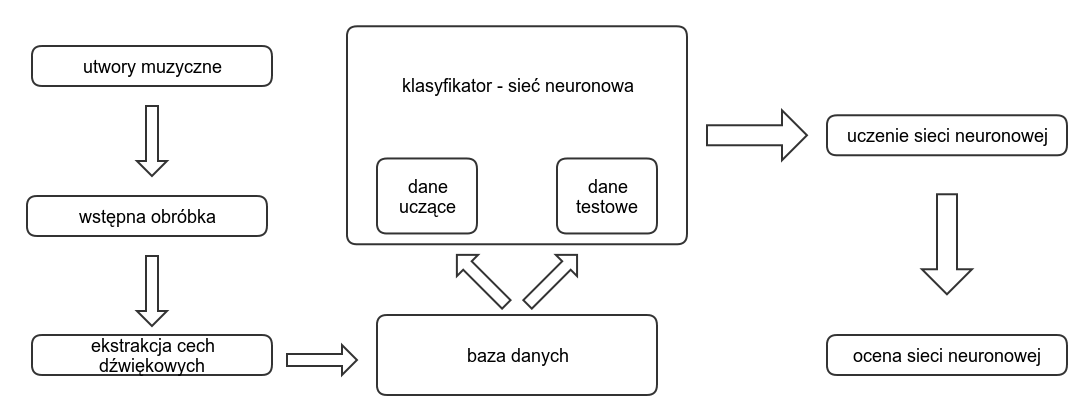
\includegraphics[scale=0.4]{res/systemScheme.png}
\caption{Schemat systemu}\label{systemSchemeImage}
\end{figure}

\subsection{Zastosowane narzędzia}
W~celu zbudowania systemu rozpoznającego nastrój muzyki należało wybrać język programowania oraz biblioteki umożliwiające analizę utworów muzycznych, ekstrakcję potrzebnych cech, a~także implementujące sztuczne sieci neuronowe. Ponadto, niezbędny był wystarczająco duży zbiór utworów muzycznych, który mógłby posłużyć jako baza danych systemu.

\subsubsection{Język programowania oraz biblioteki programistyczne}
Język programowania jest językiem w~którym człowiek może komunikować się z~komputerem i~przez to ,,kazać'' mu wykonać  określone zadanie. Niewątpliwie dobrze jest posiadać swobodę w~porozumiewaniu się tym językiem i~ten argument spowodował, że wybór padł na język programowania Python, który jest językiem wysokopoziomowym ogólnego przeznaczenia, który zdobywa coraz większą popularność. Jest to spowodowane jego prostą oraz dużymi możliwościami, co w połączeniu z~dostępnymi bibliotekami naukowymi (matplotlib, numpy) powoduje, że staje się on dużą konkurencją dla popularnego Matlaba. W parze z~językiem programowania idą także biblioteki programistyczne. W~niniejszej pracy największą rolę odegrały dwie z nich tj. biblioteka Essentia\cite{essentia} oraz NeuroLab. Pierwsza z~nich została napisana w~języku C++, ale oferuje także tzw. bindingi, które pozwalala na jej użycie także w~języku Python. Posiada ona szeroką gamę algorytmów wykorzystywanych w~analizie dźwięków i~w~tym celu została użyta w~tej pracy,a~także wielu innych związanych z MIR\footnote{MIR - Music Information Retrieval}. Druga natomiast, jest prostą i~potężną biblioteką implementującą sieci neuronowe. Obie znacznie ułatwiły pracę nad problemem podjętym w~niniejszej pracy.

\subsubsection{System operacyjny}
Systemem operacyjnym użytym przy realizacji założonego zadania był system Linux, dokładnie dystrybucja Xubuntu. Przenośność języka programowania jakim jest Python pozwala jednak na używanie aplikacji także na ich systemach pod warunkiem zainstalowania koniecznych do jego działania bibliotek jakimi są wspomniane biblioteki: Essentia oraz NeuroLab.

\subsubsection{Baza utworów muzycznych}
Koniecznością było pozyskanie odpowiedniej bazy danych, aby móc z jej wykorzystaniem nauczyć oraz przetestować sieć neuronową. Pierwszym pomysłem był odsłuch i~ocena utworów przez samego autora i~ewentualną osobę towarzyszącą. Biorąc jednak pod uwagę wysoką subiektywność percepcji muzyki prawdopodobnie nie byłby to miarodajny osąd. Z~pomocą przyszedł zbiór danych\cite{dataSet} zawierający 744 utwory różnych gatunków muzycznych opublikowany właśnie dla prac naukowych o~tematyce zbliżonej do niniejszej pracy. Wszystkie fragmenty zbioru pozyskane zostały z~otwartego archiwum muzyki\footnote{Free Music Archive - \url{http://freemusicarchive.org/}}. Każdy z~utworów jest 45-cio sekundowym fragmentem uzyskanym z~pełnego utworu oraz ocenionym zarówno pod względem pobudzenia jak i~zadowolenia przez ponad 300 osób. Skala ocen należy do przedziału $[1,9]$ dla obu parametrów, a~każdy uczestnik przeprowadzonego badania oceniał utwór w czasie ciągłym\footnote{\url{https://www.youtube.com/watch?v=G-GhONd_Wag}}, co dawało średnią częstotliwość oceniania 2~Hz biorąc pod uwagę możliwości techniczne przeglądarek internetowych oraz komputerów używanych przez badanych. Wszystko to sprawia, że ten zbiór danych stanowił dobrą podstawę dla systemu tworzonego przez autora. 

\subsubsection{Algorytm uczenia maszynowego}
Temat pracy brzmi ,,Wykorzystanie uczenia maszynowego do rozpoznawania nastroju muzyki''. Algorytmem, który jednak został wybrany do realizacji tego celu, zostały sztuczne sieci neuronowe, które pozwalają na pozostawienie problemu implementacji rozwiązania problemu samej sieci, co jest znacznym ułatwieniem.

\subsection{Opis aplikacji}
Pierwszy etapem działania programu jest wczytanie utworów muzycznych, które są zapisane w formacie mp3. Po tym następuje ich wstępna obróbka, która obejmuje zastosowanie okna czasowego dla przetwarzanego sygnału oraz algorytm wyrównywania poziomu głośności. Po wstępnej obróbce, obliczony zostaje wskaźnik zmiany znaku oraz wskaźnik zmian po której wykonywana jest transformacja Fouriera w celu otrzymania widma sygnału, które jest niezbędne w~celu obliczenia kolejnych cech dźwiękowych, którymi są kolejno złożoność spektralna, dysonans, skala, płaskość spektralna oraz kształt spektralny w którego skład wchodzą środek masy widma, współczynnik skośności widma, kurtoza widma, \emph{roll off} widma oraz rozrzut widma. Po ekstrakcji cech następuje uczenie oraz testowanie sieci neuronowej. W~tym celu baza utworów została podzielona na dwa zestawy, pierwszy z nich składa się 674 utworów służących do uczenia sieci neuronowej, natomiast drugi z 70 utworów, który służy jako zestaw do oceny sieci neuronowej. Na wejście sieci, zbudowanej z wykorzystaniem biblioteki NeuroLab, przekazywane są wyżej wymienione cechy. Jednokierunkowa sieć neuronowa (ang. \emph{feed-forward}) zwraca dwie wielkości: zadowolenie oraz pobudzenie, które opisują nastrój reprezentowany przez utwór. Wszystkie oceny badanych z wykorzystywanej bazy danych zostały przeskalowane do przedziału $[-1,1]$, ponieważ została użyta tangensoidalna funkcja aktywacji. Użycie liniowej funkcji aktywacji znacznie ogranicza możliwości sieci, co jest spowodowane tym, że funkcja modelowana przez złożenie funkcji liniowych wciąż pozostanie liniowa, natomiast funkcję liniową można modelować pojedynczym liniowym neuronem z czego wynika wniosek, że wielowarstwowa topologia zwiększa możliwości tylko w przypadku użycia nieliniowych funkcji aktywacji.

\subsection{Uczenie sieci neuronowej}
Jednym z~podstawowych zadań przy treningu sieci neuronowej jest dobór optymalnej topologii sieci, a~w~szczególności liczby neuronów w~warstwie ukrytej. Istnieją ogólne reguły jak należy w~tym wypadku postępować. 
Z~całą pewnością liczba neuronów w~warstwie ukrytej nie powinna być zbyt duża ani zbyt mała. Zbyt duża, to znaczy znacznie przekraczająca ilość neuronów wejściowych, ponieważ może to spowodować przeuczenie sieci neuronowej. Przeuczenie, lub też przetrenowanie, sieci polega na tym, że będzie ona nadmiernie dopasowana do danych uczących przez co nie będzie odporna na szumy. Można powiedzieć, że sieć nauczy się ,,na pamięć'' wyników dla danego zestawu danych, co nie jest oczekiwanym rezultatem. Zbyt mała liczba neuronów oznacza liczbę neuronów znacznie mniejszą od ilość neuronów wejściowych. Nie pozwoli to sieci odpowiednio modelować poszukiwanej zależności pomiędzy jej wejściami , a~wyjściami. W~przypadku uczenia znaczenie ma także czynnik losowy, ponieważ wagi sieci inicjalizowane są wartościami losowymi. Biorąc pod uwagę wspomniane fakty, w celu nauczenia sieci neuronowej wykonany został skrypt korzystając z języka skryptowego powłoki systemowej UNIX, który pozwalał na automatyczne wielokrotne uruchamianie programu. Korzystając z dostępnych flag sprawdzane były także wyniki uzyskiwane przez sieć dla różnej liczby neuronów w warstwie ukrytej. Użytym kryterium oceny sieci była wartość funkcji minimalizowanej przez algorytm uczący, która jest przedstawiona we wzorze \ref{minFunc}.

Na wykresie \ref{error} przedstawiona została wartość minimalizowanej funkcji w~zależności od liczby iteracji. Łatwo można zauważyć, że już od około setnej iteracji sieć neuronowa praktycznie przestaje się uczyć, następują już wtedy tylko nieznaczne zmiany. Ostatecznie, najmniejsza uzyskana wartość błędu wynosi $4.299$ dla zbioru testowego oraz $31.303$ dla zbioru uczącego. Najlepszy wynik został otrzymany dla sieci o~liczbie neuronów w~warstwie ukrytej równej 7. Łatwo jest jest też doprowadzić do sytuacji przeuczenia sieci. W przypadku uruchomienia programu z~40~neuronami w~warstwie ukrytej otrzymujemy błędy $13.426$; $10.575$ kolejno dla zestawu uczącego oraz testowego. Jak łatwo zauważyć, pomimo tego, że mogłoby się wydawać, że sieć dużo lepiej została wytrenowana, to jedna wyniki dla zestawu testowego są gorsze niż w~przypadku tej pozornie gorzej wytrenowanej. W tabeli \ref{table:przeuczenie} przedstawione zostały wartości błędu dla zestawów uczących oraz testowych dla sieci z 40 neuronami oraz z~7~neuronami podzielone przez liczbę utworów uczących oraz testowych. Widać tutaj sporą różnicę pomiędzy błędem dla zestawu testowego oraz uczącego w~przypadku sieci z 40 neuronami, co wskazuje zdecydowanie na jej przeuczenie.

\begin{table}
\centering
\begin{tabular}{|c|c|c|}
\hline
 liczba neuronów sieci & 40 & 7 \\ 
 \hline
% błąd dla 70 utworów uczących & $1.38$ & $3.445$ \\  
błąd dla utworów uczących / liczba utworów uczących & $0,012$ & $0.050$ \\  
 \hline
% błąd dla 70 utworów testowych & $10.575$ & $4.299$ \\ 
błąd dla utworów testowych / liczba utworów testowych & $0.15$ & $0.061$ \\ 
 \hline  
 \end{tabular}
 \caption{Błąd dla 70 utworów dwóch różnych sieci} \label{table:przeuczenie}
\end{table}


\begin{figure}[ht!]
\centering
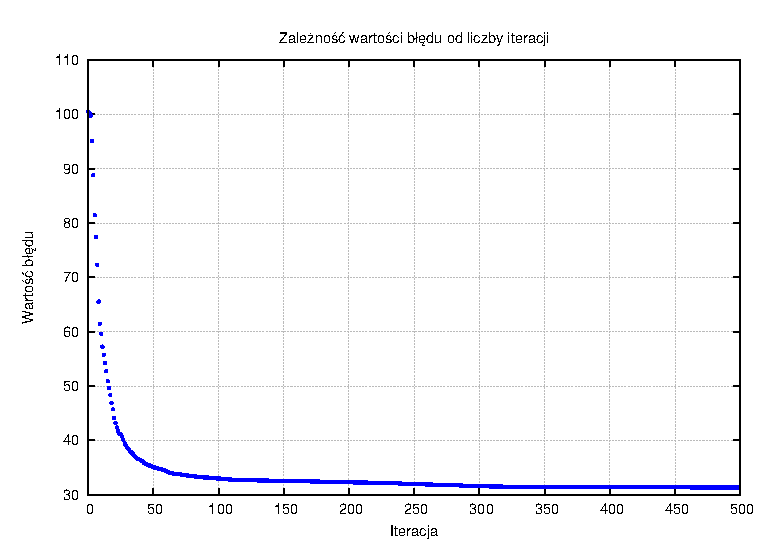
\includegraphics[scale=1.27]{res/error.eps}
\caption{Zależność wartości błędu od liczby iteracji\label{error}}
\end{figure}


\section{Uzyskane wyniki}\label{rozdzial_wyniki}
\newcommand{\imageSize}{1.15}
\subsection{Parametry zadowolenia oraz pobudzenia}
Zależność pomiędzy odpowiedziami oczekiwanymi przez sieć, a~jej rzeczywistymi odpowiedziami, w~przypadku dobrze nauczonej i~działającej sieci powinna być zbliżona do liniowej. Biorąc to pod uwagę, przedstawiono wykresy, których jedna oś wskazuje oczekiwaną wartość parametru, a~druga rzeczywistą wartość parametru w celu zaobserwowania czy występuję liniowość, co też uczyniono, a efekty można zaobserwować na rysunkach \ref{arousal} oraz \ref{valence}. Jak można zauważyć, istnieje pewna korelacja dla obu parametrów. W~celu określenia konkretnych wartości liczbowych wskazujących na korelację możemy posłużyć się współczynnikiem korelacji liniowej zmiennych $x$ oraz $y$, który wyraża się wzorem:
\begin{equation}
\rho_{xy} = \frac{cov(x,y)}{\sigma_x \sigma_y},
\end{equation}
gdzie $\sigma_x$, $\sigma_y$ są odchyleniami standardowymi odpowiednio $x$ oraz $y$, natomiast $cov(x,y)$ jest kowariancją i określamy ją wzorem:
\begin{equation}
cov(x,y) = \overline{xy} - \overline{x}*\overline{y},
\end{equation}
gdzie $\overline{xy}$, $\overline{x}$, $\overline{y}$ są kolejno wartościami średnimi $xy$, $x$ oraz $y$.
Obliczone współczynniki korelacji przedstawiono w~tabeli \ref{table:coeff}.
Zaobserwowana korelacja nie jest zbyt duża, niemniej jednak widzimy wyraźny związek pomiędzy odpowiedzią sieci neuronów, a~wartościami pobudzenia oraz zadowolenia wyznaczonymi przez badane osoby. Biorąc pod uwagę subiektywny
charakter oceny nastroju przez człowieka, jak również fakt, że sieć neuronowa używała tylko 11 cech uzyskanych z danego utworu muzyki, jest to wynik świadczący tym, że przedstawiony system do pewnego stopnia reprodukuje subiektywne oceny ludzi.
\begin{table}
\centering
\begin{tabular}{|c|c|c|}
\hline
 parametr & zadowolenie & pobudzenie \\ 
\hline
 współczynnik korelacji & $0.66$ & $0.55$ \\  
\hline 
\end{tabular}
\caption{Współczynniki korelacji liniowych parametrów zadowolenia oraz pobudzenia} \label{table:coeff}
\end{table}


\begin{figure}[ht!]
\centering
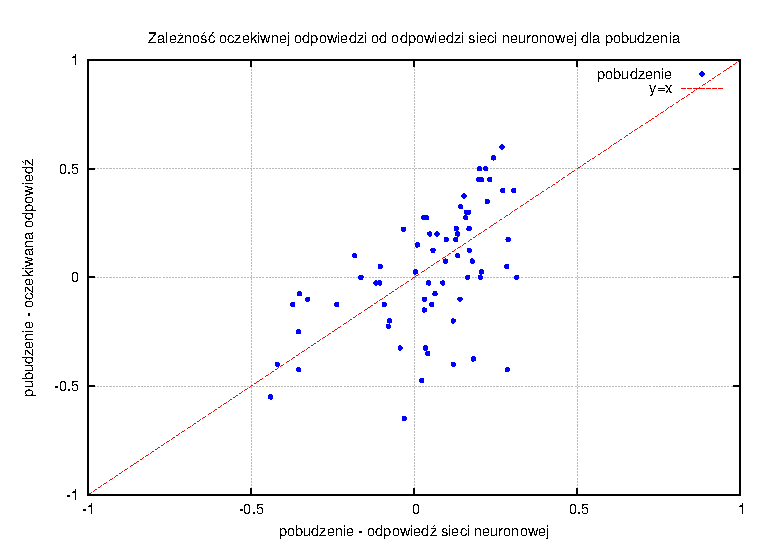
\includegraphics[scale=\imageSize]{res/arousal.eps}
\caption{Zależność oczekiwanej odpowiedzi od odpowiedzi sieci neuronowej dla parametru pobudzenia\label{arousal}}
\end{figure}

\begin{figure}[ht!]
\centering
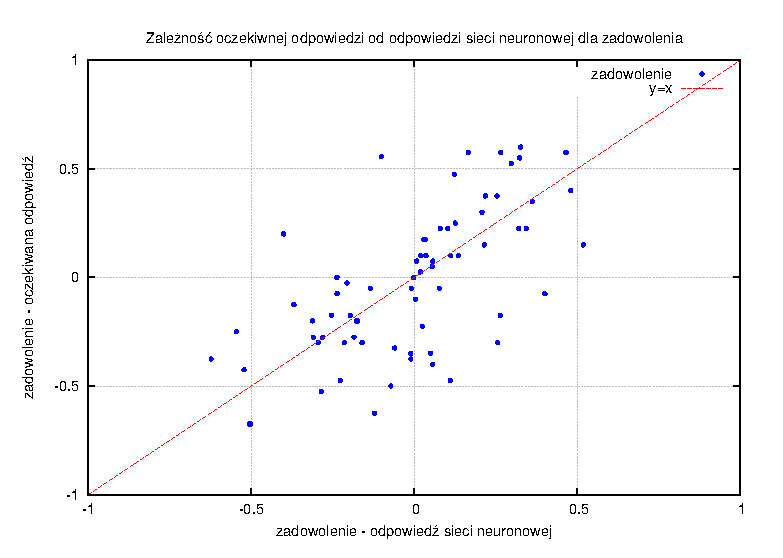
\includegraphics[scale=\imageSize]{res/valence.eps}
\caption{Zależność oczekiwanej odpowiedzi od odpowiedzi sieci neuronowej dla parametru zadowolenia\label{valence}}
\end{figure}


\subsection{Zależność nastroju od cech dźwiękowych}\label{rozdzial_zaleznosc}
Pod uwagę zostało wziętych 11 cech dźwiękowych, które mają różny wpływ na subiektywny nastrój reprezentowany przez utwór muzyczny. W~tym rozdziale przeanalizowana jest zależność wartości parametrów zadowolenia oraz pobudzenia od wartości cech dźwiękowych. 


%%%%%%%%%%%%%%%%%%%%%%%%%%%%%%%%%%%%%%%%%%%%%%%%%%%%%%%%
\paragraph{Wskaźnik zmiany znaku}\mbox{}\\
\begin{minipage}{\textwidth}
Rysunek \ref{wykresCrossRate} przedstawia zależność wskaźnika zmiany znaku od subiektywnej oceny zadowolenia oraz pobudzenia. Możemy zaobserwować tendencję, że wraz ze wzrostem wartości tego wskaźnika wzrasta również wartość obu parametrów - zadowolenia jak i~pobudzenia. Nie jest to jednak znaczący wzrost.
\end{minipage}
\begin{figure}[ht!]
\centering
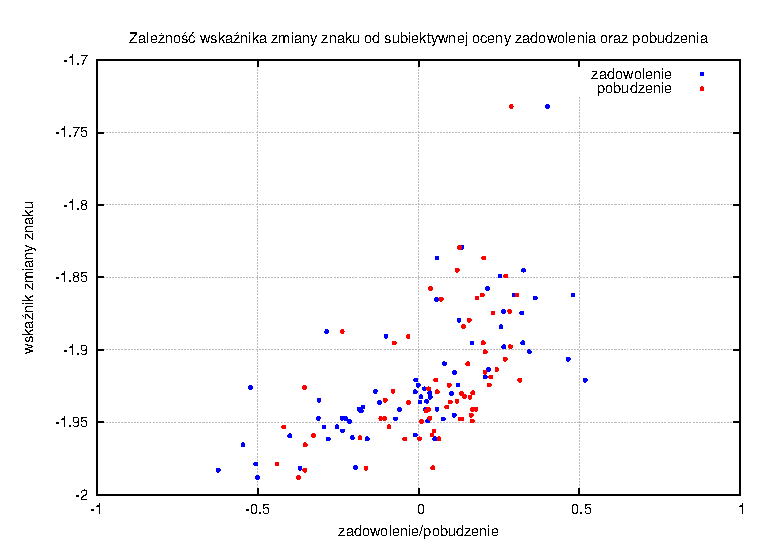
\includegraphics[scale=\imageSize]{res/crossRate.eps}
\caption{Zależność wskaźnika zmiany znaku od subiektywnej oceny zadowolenia (punkty niebieskie) oraz pobudzenia (punkty czerwone)\label{wykresCrossRate}}
\end{figure}
%%%%%%%%%%%%%%%%%%%%%%%%%%%%%%%%%%%%%%%%%%%%%%%%%%%%%%%%
\paragraph{Wskaźnik zmian}\mbox{}\\
Podobnie jak w przypadku wskaźnika zmiany znaku, oba parametry - zadowolenie oraz pobudzenie wzrastają nieznacznie wraz ze wzrostem wskaźnika zmian, ale wzrost ten jest nieznaczny. Wykres przedstawiony jest na rysunku \ref{wykresOnset}.
\begin{figure}[ht!]
\centering
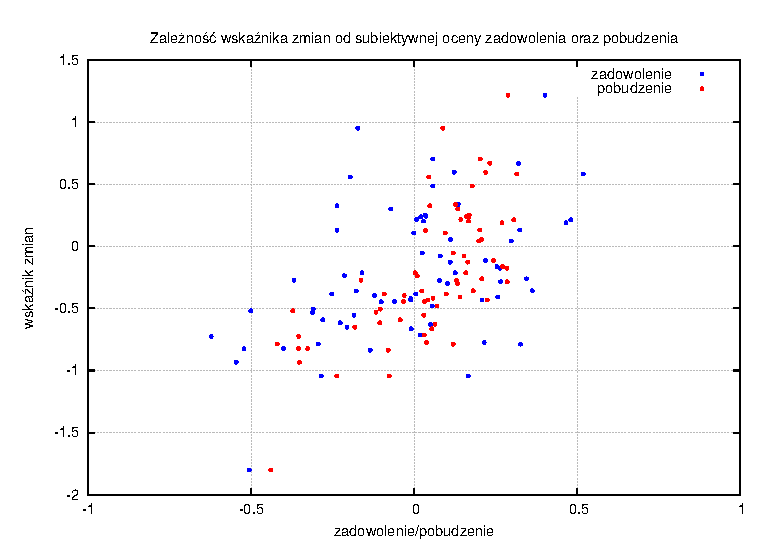
\includegraphics[scale=\imageSize]{res/onset.eps}
\caption{Zależność wskaźnika zmian od subiektywnej oceny zadowolenia (punkty niebieskie) oraz pobudzenia (punkty czerwone)\label{wykresOnset}}
\end{figure}
%%%%%%%%%%%%%%%%%%%%%%%%%%%%%%%%%%%%%%%%%%%%%%%%%%%%%%%%
\paragraph{Złożoność spektralna}\mbox{}\\
Zależność parametrów wskazujących na emocje od złożoności spektralnej została przedstawiona na rysunku \ref{wykresComplexity}. Obserwując wykres trudno mówić o~jakiejkolwiek korelacji. Zdecydowana większość wartości wydaje być się losowo rozrzucona.
\begin{figure}[ht!]
\centering
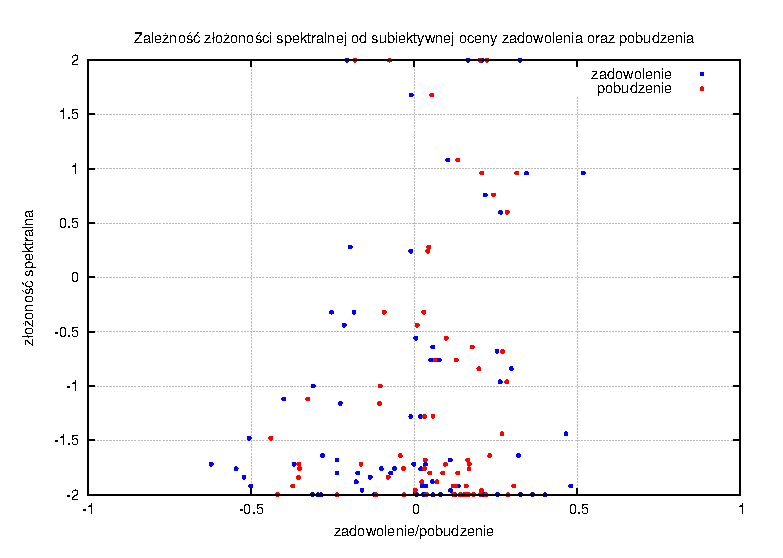
\includegraphics[scale=\imageSize]{res/complexity.eps}
\caption{Zależność złożoności spektralnej od subiektywnej oceny zadowolenia (punkty niebieskie) oraz pobudzenia (punkty czerwone)\label{wykresComplexity}}
\end{figure}


%%%%%%%%%%%%%%%%%%%%%%%%%%%%%%%%%%%%%%%%%%%%%%%%%%%%%%%%
\paragraph{Środek masy widma}\mbox{}\\
W~przypadku środka masy widma możemy zauważyć nieznaczny związek pomiędzy zmianą wartości środka widma, a~parametrami zadowolenia oraz pobudzenia. Zostało to przedstawione na rysunku \ref{wykresCentroid}.
\begin{figure}[ht!]
\centering
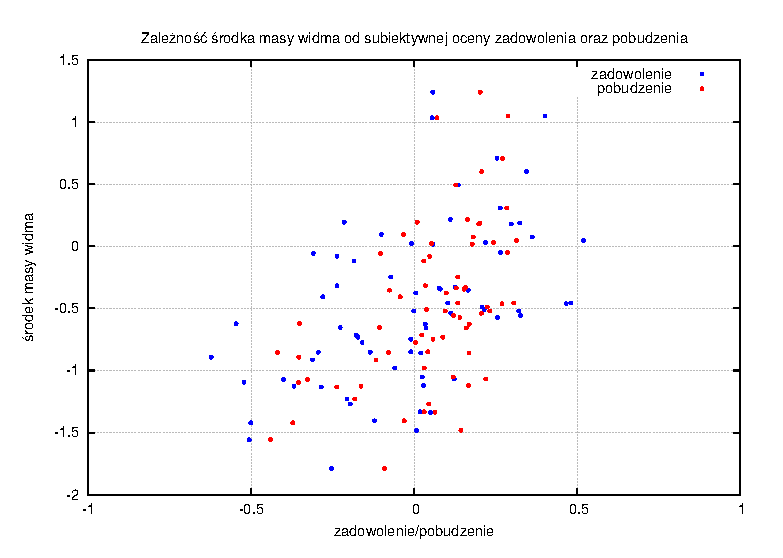
\includegraphics[scale=\imageSize]{res/centroid.eps}
\caption{Zależność środa masy widma od subiektywnej oceny zadowolenia (punkty niebieskie) oraz pobudzenia (punkty czerwone)\label{wykresCentroid}}
\end{figure}
%%%%%%%%%%%%%%%%%%%%%%%%%%%%%%%%%%%%%%%%%%%%%%%%%%%%%%%%
\paragraph{Współczynnik skośności widma}\mbox{}\\
Jeśli chodzi o~współczynnik skośności widma możemy zaobserwować, że przy wyższych jego wartościach parametry bardzo nieznacznie mogą być zwiększone, co jednak także nie jest wyraźne i~przedstawia się na wykresie \ref{wykresSkewness}.
\begin{figure}[ht!]
\centering
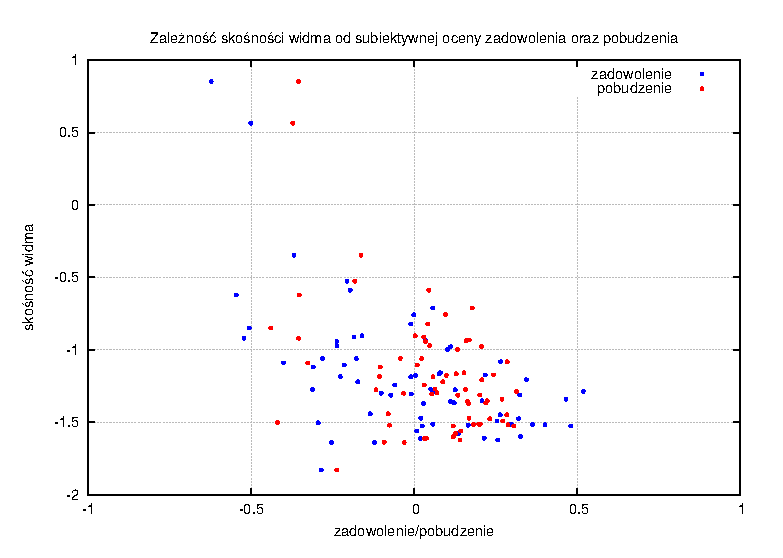
\includegraphics[scale=\imageSize]{res/skewness.eps}
\caption{Zależność skośności widma od subiektywnej oceny zadowolenia (punkty niebieskie) oraz pobudzenia (punkty czerwone)\label{wykresSkewness}}
\end{figure}
%%%%%%%%%%%%%%%%%%%%%%%%%%%%%%%%%%%%%%%%%%%%%%%%%%%%%%%%
\paragraph{Kurtoza widma}\mbox{}\\
Kurtoza widma według wykresu \ref{wykresKurtosis} nie wydaje się mieć większego wpływu na wartości parametrów zadowolenia oraz pobudzenia.
\begin{figure}[ht!]
\centering
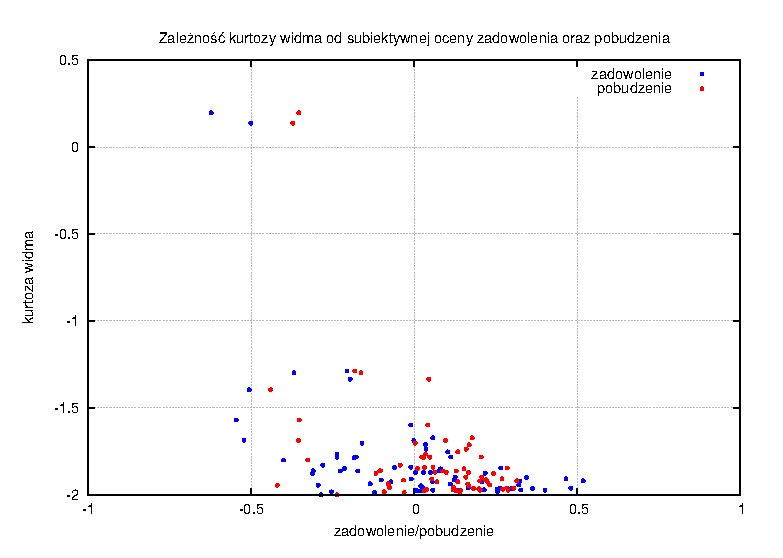
\includegraphics[scale=\imageSize]{res/kurtosis.eps}
\caption{Zależność kurtozy widma od subiektywnej oceny zadowolenia (punkty niebieskie) oraz pobudzenia (punkty czerwone)\label{wykresKurtosis}}
\end{figure}
%%%%%%%%%%%%%%%%%%%%%%%%%%%%%%%%%%%%%%%%%%%%%%%%%%%%%%%%
\paragraph{Rozrzut spektralny}\mbox{}\\
Rozrzut spektralny przedstawiony na wykresie \ref{wykresSpread} wydaje się być względnie znaczącym czynnikiem w~ocenie parametrów nastroju muzyki w~stworzonym systemie. Oba z~nich wzrastają w~przypadku wzrosty wartości tej cechy dźwięku.
\begin{figure}[ht!]
\centering
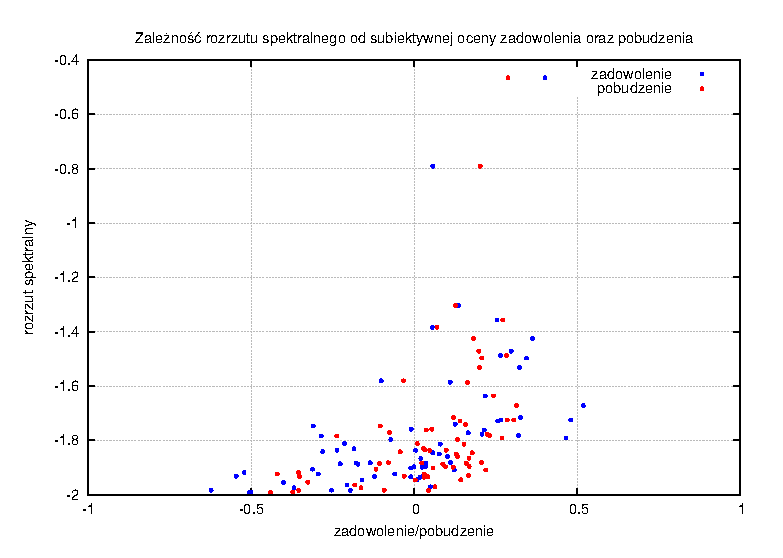
\includegraphics[scale=\imageSize]{res/spread.eps}
\caption{Zależność rozrzutu spektralnego od subiektywnej oceny zadowolenia (punkty niebieskie) oraz pobudzenia (punkty czerwone)\label{wykresSpread}}
\end{figure}
%%%%%%%%%%%%%%%%%%%%%%%%%%%%%%%%%%%%%%%%%%%%%%%%%%%%%%%%
\paragraph{\emph{Roll-off} widma}\mbox{}\\
Zależność \emph{Roll off}u widma od parametrów pobudzenia oraz zadowolenia nie wskazuje na większą korelację (patrz Rys.~\ref{wykresRollOff}).
\begin{figure}[ht!]
\centering
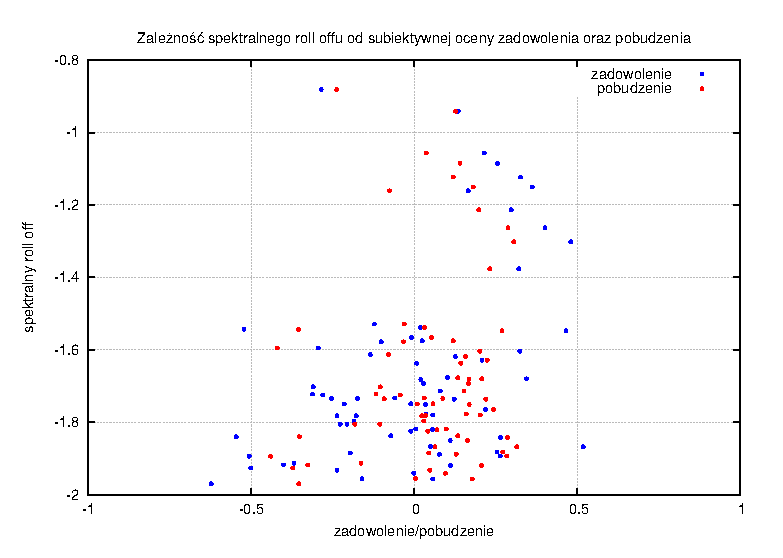
\includegraphics[scale=\imageSize]{res/rollOff.eps}
\caption{Zależność spektralnego \emph{roll off}'u od subiektywnej oceny zadowolenia (punkty niebieskie) oraz pobudzenia (punkty czerwone)\label{wykresRollOff}}
\end{figure}
%%%%%%%%%%%%%%%%%%%%%%%%%%%%%%%%%%%%%%%%%%%%%%%%%%%%%%%%
\paragraph{Płaskość spektralna}\mbox{}\\
Na wykresie \ref{wykresFlatness} przedstawiony został wpływ parametru płaskości spektralnej na parametry pobudzenia oraz zadowolenia. Również i~w~tym przypadku nie widać większych korelacji.
\begin{figure}[ht!]
\centering
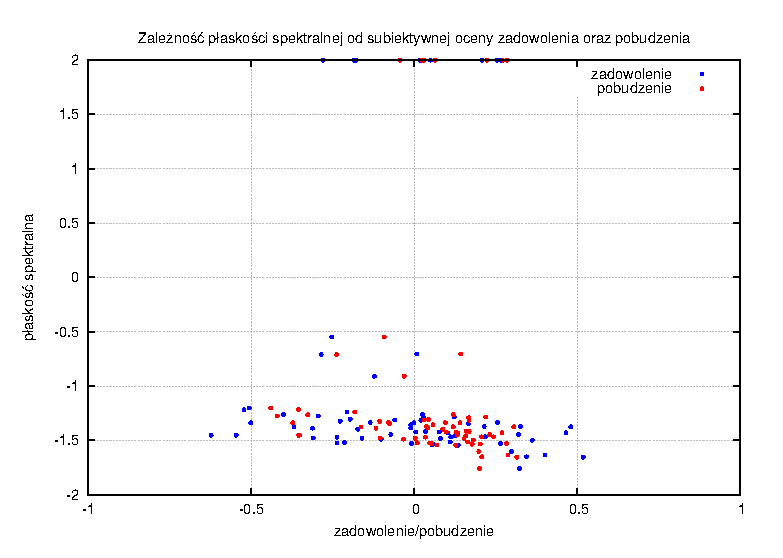
\includegraphics[scale=\imageSize]{res/flatness.eps}
\caption{Zależność płaskości spektralnej od subiektywnej oceny zadowolenia (punkty niebieskie) oraz pobudzenia (punkty czerwone)\label{wykresFlatness}}
\end{figure}

%%%%%%%%%%%%%%%%%%%%%%%%%%%%%%%%%%%%%%%%%%%%%%%%%%%%%%%%
\paragraph{Dysonans}\mbox{}\\
Podobnie jak w przypadku płaskości spektralnej nie istnieje większa korelacja pomiędzy parametrami nastroju muzyki, a~dysonansem, co wizualizuje wykres\ref{wykresDissonance}.
\begin{figure}[ht!]
\centering
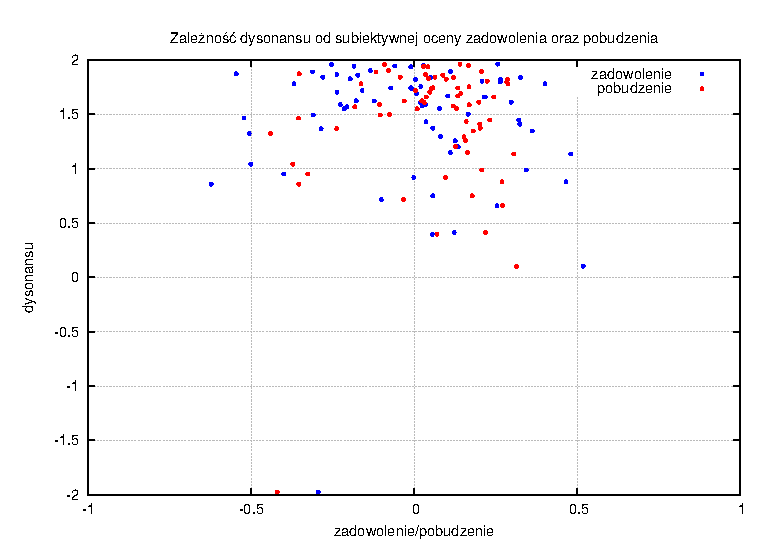
\includegraphics[scale=\imageSize]{res/dissonance.eps}
\caption{Zależność dysonansu od subiektywnej oceny zadowolenia (punkty niebieskie) oraz pobudzenia (punkty czerwone)\label{wykresDissonance}}
\end{figure}

%%%%%%%%%%%%%%%%%%%%%%%%%%%%%%%%%%%%%%%%%%%%%%%%%%%%%%%%
\paragraph{Skala}\mbox{}\\
W~tabeli \ref{table:scale} zostały przedstawione średnie wartości pobudzenia oraz zadowolenia dla skali muzycznych majorowej oraz minorowej, które jednak zbliżone są bardzo do siebie w przypadku obu skal. Sugeruje to, że ta cecha dźwiękowa nie była dobrym wskaźnikiem jeśli chodzi o~parametry pobudzenia oraz zadowolenia. 
\begin{table}
\centering
\begin{tabular}{|c|c|c|}
\hline
 skala & minorowa (molowa) & majorowa (durowa) \\ 
\hline
 wartość średnia dla zadowolenia & $0.02 \pm 0.25$ & $-0.08 \pm 0.30$ \\  
\hline 
 wartość średnia dla pobudzenia & $0.06 \pm 0.19$ & $0.03 \pm 0.19$ \\  
\hline 
\end{tabular}
\caption{Wartości średnie dla skali muzycznej wraz z odchyleniem standardowym} \label{table:scale}
\end{table}
\paragraph{Podsumowanie}\mbox{}\\
Obserwując wykresy dla poszczególnych cech dźwiękowych nie jest trudno dojść do wniosku, że nie wszystkie z~nich mają wpływ na parametry nastroju muzyki, a~te które mają, nie są silnymi zmiennymi. Tłumaczy to niezbyt wysoką korelację przedstawioną w~tabeli \ref{table:coeff}. Analiza utworów została przeprowadzona powtórnie, ale biorąc pod uwagę tylko te cechy, które korelowały z~wartościami pobudzenia oraz zadowolenia czyli: wskaźnik zmiany znaku, wskaźnik zmian, środek masy widma, skośność spektralną oraz rozrzut spektralny. Otrzymane rezultaty przedstawia tabela \ref{table:coeff2} oraz wykresy \ref{arousal2} i \ref{valence2}. Jak widać, usunięcie kilku zmiennych i pozostawienie tylko znaczących cech nie wpłynęło w~wyraźny sposób na wyniki reprezentowane przez współczynniki korelacji. Świadczy to o~tym, że na końcowy wynik efektywny wpływ ma tylko 5 pozostawionych cech.

\begin{table}
\centering
\begin{tabular}{|c|c|c|}
\hline
 parametr & zadowolenie & pobudzenie \\ 
\hline
 współczynnik korelacji & $0.54$ & $0.58$ \\  
\hline 
\end{tabular}
\caption{Współczynniki korelacji liniowych parametrów zadowolenia oraz pobudzenia} \label{table:coeff2}
\end{table}

\begin{figure}[ht!]
\centering
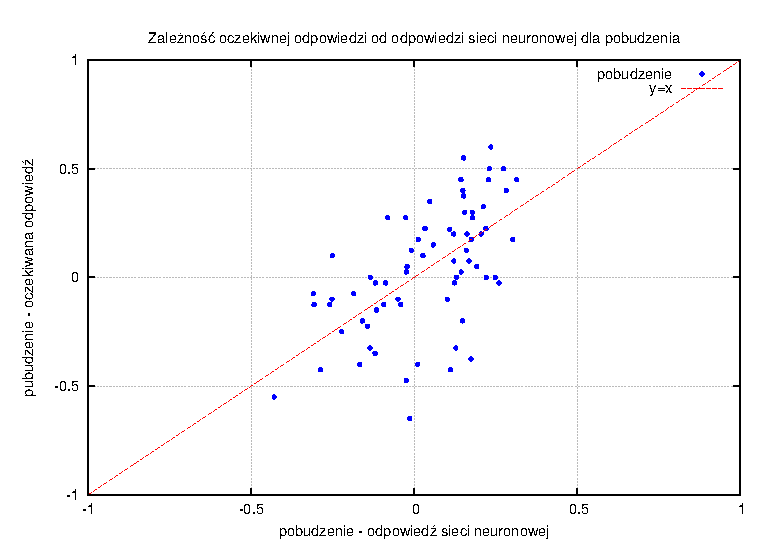
\includegraphics[scale=\imageSize]{res/arousal2.eps}
\caption{Zależność oczekiwanej odpowiedzi od odpowiedzi sieci neuronowej dla parametru pobudzenia\label{arousal2}}
\end{figure}

\begin{figure}[ht!]
\centering
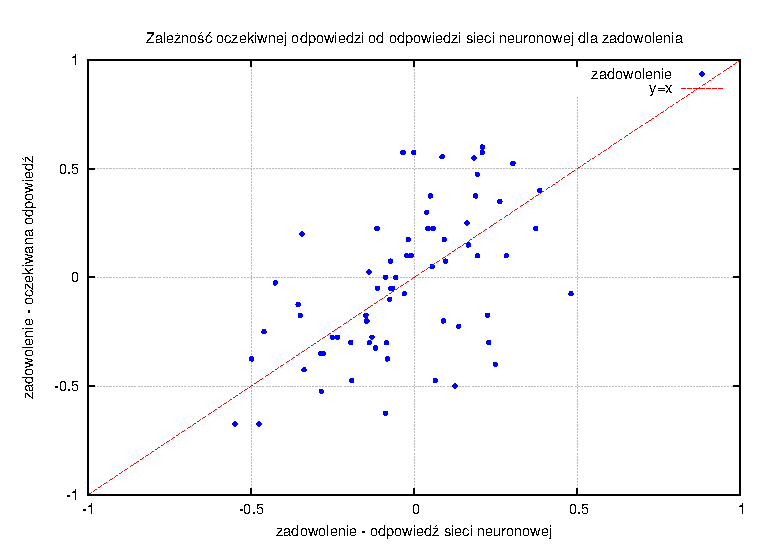
\includegraphics[scale=\imageSize]{res/valence2.eps}
\caption{Zależność oczekiwanej odpowiedzi od odpowiedzi sieci neuronowej dla parametru zadowolenia\label{valence2}}
\end{figure}






\section{Wnioski}\label{rozdzial_wnioski}
\subsection{Ocena działania systemu}
System do pewnego stopnia spełnił postawione przed nim zadania. Otrzymane wyniki pokazują, że stworzona sieć neuronowa nie modeluje w~znaczącym stopniu zależności pomiędzy cechami dźwiękowymi utworów muzycznych, a~parametrami określającymi nastrój tych utworów. Współczynniki przedstawione w~tabeli \ref{table:coeff} wskazują na słabą korelację pomiędzy odpowiedziami sieci, a~oczekiwanymi wartościami. Można jednak zaobserwować pewną korelację pomiędzy uzyskaną przez system oceną nastroju, a~oceną badanych. Wskazuje to, że możliwe jest zbudowanie efektywnego systemu klasyfikującego. Po lekturze rozdziału \ref{rozdzial_zaleznosc} zauważamy, że jedynie 5 z 11 analizowanych cech daje podstawy dla sieci pozwalające wyznaczyć wartości pobudzenia oraz zadowolenia, co nie wątpliwie jest jedną z przyczyn niskich współczynników korelacji. Należy jednak zauważyć, że wszystkie utwory były analizowane całościowo tzn. sygnał nie był dzielony na mniejsze fragmenty, co prawdopodobnie jest przyczyną niezadowalających wyników. Nastrój muzyki zmienia się w czasie, co także powinno być wzięte pod uwagę w przypadku realizacji zadania rozpoznawania emocji reprezentowanych przez muzykę, co zostało zrobione w~innych pracach podejmujących podobną tematykę\cite{musicANN1}\cite{musicANN2} i~dało wyraźnie lepsze rezultaty. Należy jednak mieć na uwadze jednak także bazę danych na której przeprowadzono badania, gdyż duże znaczenie może mieć także jej zróżnicowanie pod kątem gatunków muzycznych. 
\subsection{Propozycja usprawnienia}
Biorąc pod uwagę wspominane prawdopodobne przyczyny niskiej efektywności systemu, pierwszą, najważniejszą propozycją usprawnienia jest dzielenie sygnału audio na mniejsze fragmenty, ocena ich oraz uśrednienie wyników, co mogłoby dać lepsze wyniki. Należałoby wtedy także przekonać się czy cechy dźwięku wykorzystane w programie wciąż nie mają wpływu na wartości parametrów zadowolenia oraz pobudzenia, a~także rozważyć użycie innych cech, co nie stanowiłoby wielkiego wyzwania dzięki bibliotece programistycznej Essentia, gdyż oferuje ona kilkadziesiąt możliwych do wykorzystania algorytmów. Oprócz cech wynikających z~samego sygnału audio, możliwe jest także analiza tekstu utworów, który również ma znaczący wpływ na nastrój utworu. Dodatkową sugestią w kwestii rozpoznawania nastroju mogą być także okładki płyt z których pochodzą utwory muzyczne, co również mogłoby usprawnić ocenę. Innym kierunkiem rozwoju aplikacji prezentowanej w pracy jest także ocena utworów muzycznych pod kątem ich gatunków.
\clearpage
\addcontentsline{toc}{section}{Literatura}
\bibliography{bibliography}{}
\bibliographystyle{unsrt}

%\section{Podsumowanie}\label{podsumowanie}
%Zadanie rozpoznawania emocji reprezentowanych przez muzykę jest niewątpliwie wymagające, a jego tematyka wiąże się z %wieloma dziedzinami nauki. Pomimo tego, nie jest ono nieosiągalne i również ta praca pokazuje, że jest możliwe %stworzenie efektywnie działającego systemu klasyfikacji, który bierze pod uwagę emocje reprezentowane przez utwór %muzyczny.

\renewcommand{\appendixtocname}{Dodatki}
\renewcommand{\appendixpagename}{Dodatki}

\begin{appendices}
\section{Obsługa programu}
\subsection{Konfiguracja}
Stworzony program posiada możliwości konfiguracyjne. W~celu edycji ustawień należy edytować plik Configurations.py, który zawiera szereg stałych, których zdefiniowanie jest konieczne do poprawnego działania aplikacji. Większość z~nich są to ścieżki do plików, którymi są m.in. ścieżki dostępu do utworów muzycznych, oceny utworów muzycznych czy też ścieżka do pliku przechowującego logi uruchomienia oraz format samego logowania wiadomości. Można znaleźć tam także szczegóły konfiguracyjne dotyczące samej sieci neuronowej tj. liczba neuronów w~warstwie ukrytej oraz liczba wyjść w zależności od potrzeb. 

\subsection{Uruchamianie}
Wykonany program pozwala na uruchamianie go w~różnych trybach w~zależności od potrzeb. Podczas działania programu do konsoli wypisywane są logi, które informują użytkownika o tym co dzieje się w danym momencie lub co poszło nie tak w~razie, gdy taka sytuacja nastąpi. Podstawowy przepływ jeśli chodzi o działanie aplikacji jest zgodny ze schematem systemu przedstawionym na rysunku\ref{systemSchemeImage}. Korzystając jednak z~odpowiednich flag możemy go modyfikować. Jednym z~dłużej trwających procesów podczas wykonywania jest ekstrakcja cech dźwiękowych z~utworów ze względu na ich dużą ilość. Z tego względu możliwe jest podanie przy uruchomieniu flagi -a, która pozwala określić czy chcemy analizować wszystkie piosenki czy wczytać je z~pliku o ile taki istnieje. Jego ścieżka znajduje się w~pliku konfiguracyjnym. Po każdym uruchomieniu programu przeanalizowane cechy dźwiękowe są zapisywane do pliku, więc program należy przynajmniej raz uruchomić z~flagą -a. Użyteczną flagą jest także flaga -t, która pozwala na wczytanie sieci neuronowej, ale także tyle wtedy, gdy istnieje plik wskazany w konfiguracji. Podobnie jak w przypadku flagi -a, należy przynajmniej raz uruchomić program z~flagą -t, aby stworzyć chociaż jedną sieć neuronową.
Inne dostępne flagi, których możemy użyć prezentują się następująco:
\begin{itemize}
\item -h, --help wyświetlenie pomocy
\item -n N, określenie ilości neuronów $N$ w warstwie ukrytej dla nowej sieci neuronowej (należy używać tylko w połączeniu z flagą -t)
\item -e, ocena sieci neuronowej dla zbioru testowego
\item -p, rysowanie wykresów dla parametrów zadowolenia oraz pobudzenia (należy używać tylko w połączeniu z flagą -e)
\item -s FILE, ocena utworu muzycznego znajdującego się pod ścieżką FILE pod względem parametrów zadowolenia oraz pobudzenia (należy używać bez innych flag)
\end{itemize}
\end{appendices}
\end{document}

% notatki co trzeba się dowiedzieć przed obroną lepiej
% cel procesu uczenia i metoda najmniejszej kwadratów
% bias -> Po co to i na co to -->http://galaxy.agh.edu.pl/~vlsi/AI/bias/bias.html http://stackoverflow.com/questions/2480650/role-of-bias-in-neural-networks
% dowiedziec sie cos o uczeniu bez nauczyciela?